        	\begin{question}{1200}{Trigonométrie}{1}{31}
				Quel est le sinus de $\frac{2\pi}{3}$?
            \end{question}
            \begin{reponses}
            	\item[true] $\frac{\sqrt{3}}{2}$
            	\item[false] $\frac{\sqrt{2}}{2}$
                \item[false] 1
                \item[false] $1/2$
            \end{reponses}
			%%%%%%%%%%%%%%%%%%%%%%%%%%%%%%%%%%%%%
            \begin{question}{1200}{Trigonométrie}{2}{31}
                Que valent le cosinus et le sinus de l'angle représenté ci-dessous?
                \begin{center}
                	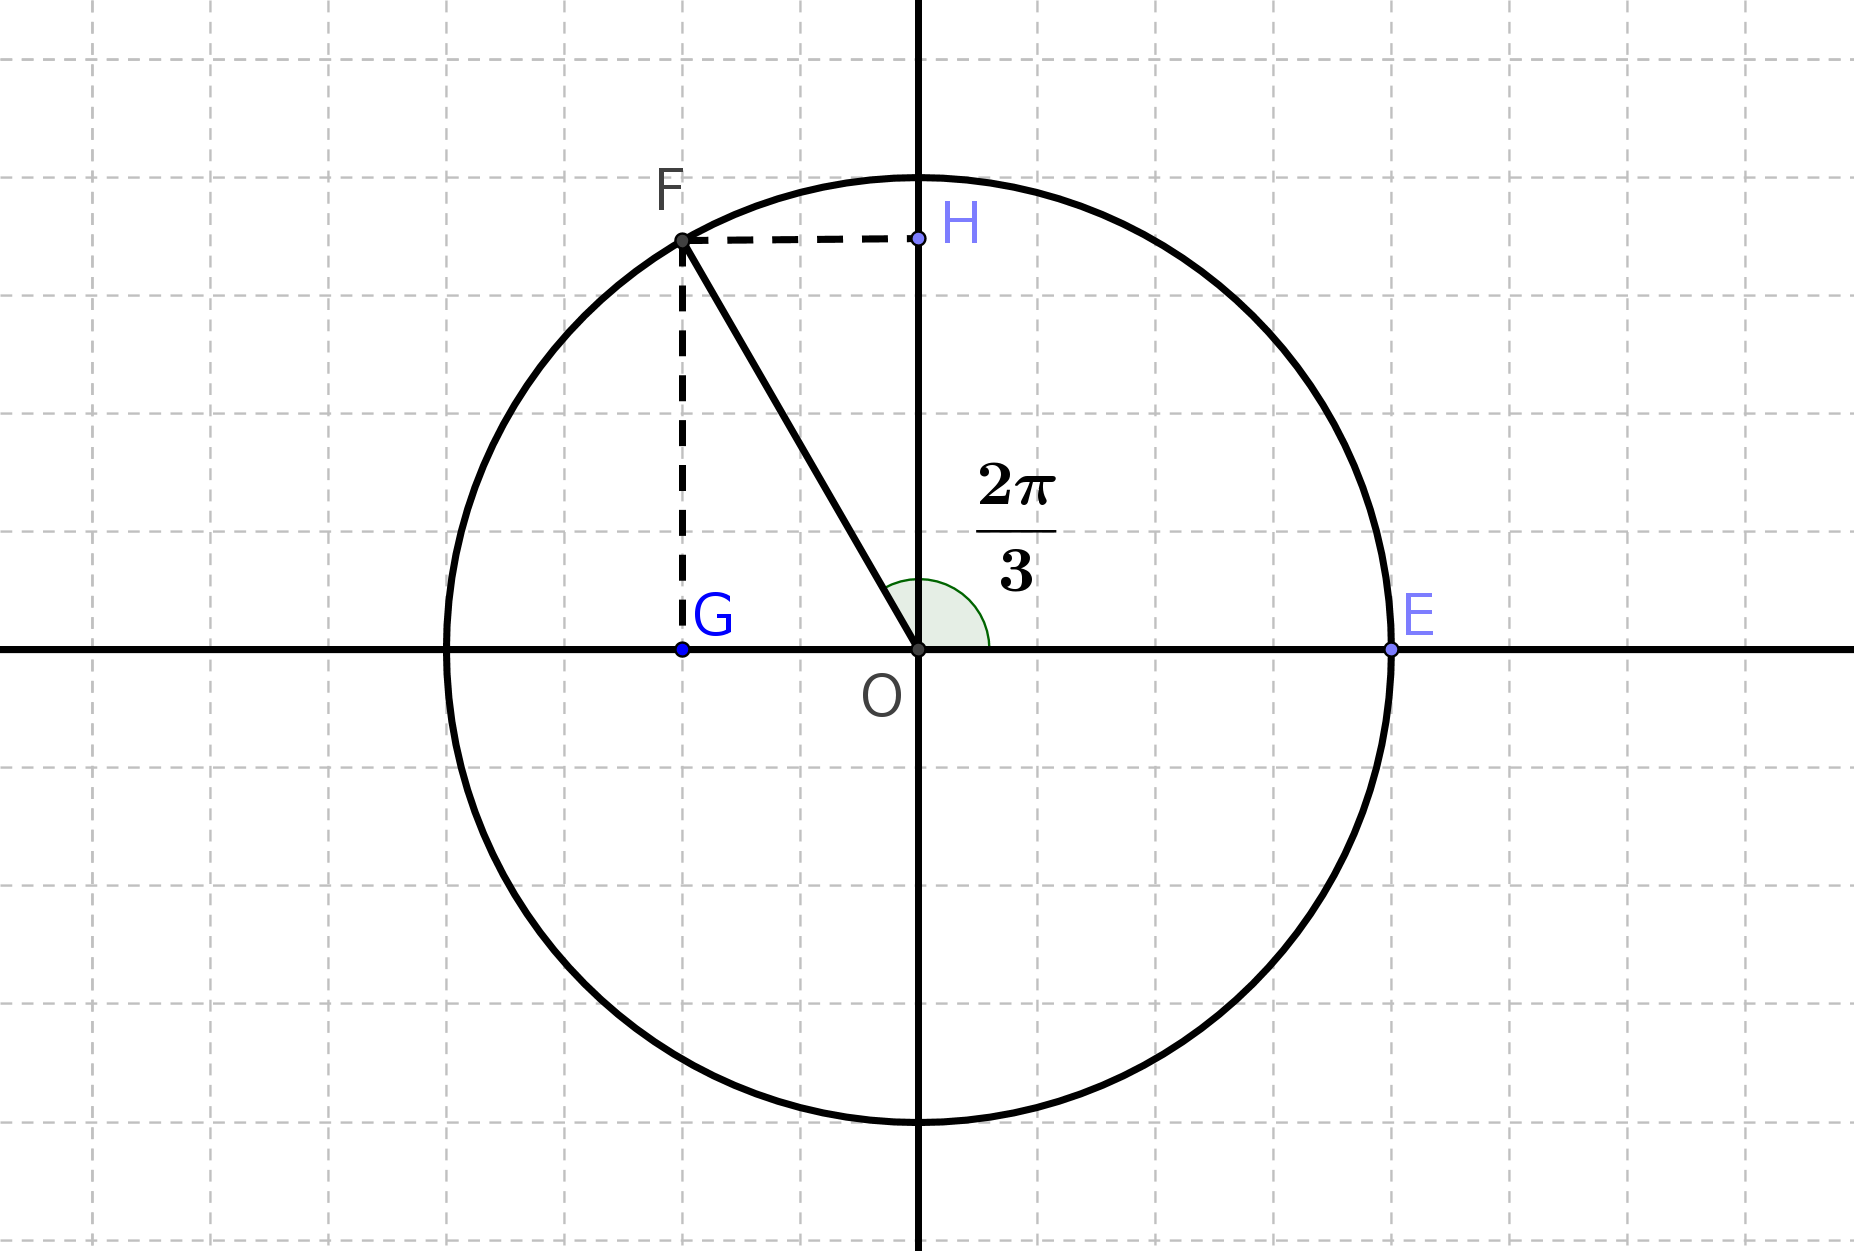
\includegraphics[width=0.5\textwidth]{Philippe/Figures_Philippe/trigo_1_4.png}
                \end{center}
            \end{question}
            \begin{reponses}
                \item[true] $\cos = -\frac{1}{2}$ et $\sin = \frac{\sqrt{3}}{2}$
                \item[false] $\cos = \frac{1}{2}$ et $\sin = \frac{\sqrt{3}}{2}$
                \item[false] $\cos = \frac{\sqrt{3}}{2}$ et $\sin = \frac{1}{2}$
                \item[false] $\cos = -\frac{\sqrt{3}}{2}$ et $\sin = \frac{1}{2}$
            \end{reponses}
            %%%%%%%%%%%%%%%%%%%%%%%%%%%%%%%%%%%%%
        	\begin{question}{1200}{Trigonométrie}{2}{31}
				Parmi ces angles, lequel a pour sinus $0,5$?
            \end{question}
            \begin{reponses}
            	\item[false] $\frac{2\pi}{3}$
            	\item[false] $\frac{3\pi}{4}$
                \item[true] $\frac{5\pi}{6}$
                \item[false] $\pi$
            \end{reponses}
			%%%%%%%%%%%%%%%%%%%%%%%%%%%%%%%%%%%%%
        	\begin{question}{1200}{Trigonométrie}{2}{31}
				Une force fait un angle $\theta$ avec la verticale. Cet angle a pour cosinus $\frac{\sqrt{2}}{2}$. Parmi les angles suivants, duquel s'agit-il?
            \end{question}
            \begin{reponses}
            	\item[true] $-\frac{\pi}{4}$
            	\item[false] $\frac{3\pi}{4}$
                \item[false] $\frac{5\pi}{4}$
                \item[false] $-\frac{3\pi}{4}$
            \end{reponses}
			%%%%%%%%%%%%%%%%%%%%%%%%%%%%%%%%%%%%%
            \begin{question}{1200}{Trigonométrie}{3}{31}
                Parmi ces angles, lequel a pour sinus $-0,5$?
            \end{question}
            \begin{reponses}
                \item[false] $\frac{4\pi}{3}$
                \item[true] $\frac{11\pi}{6}$
                \item[false] $\frac{5\pi}{3}$
                \item[false] $\frac{9\pi}{6}$
            \end{reponses}
            %%%%%%%%%%%%%%%%%%%%%%%%%%%%%%%%%%%%%
            \begin{question}{1200}{Trigonométrie}{3}{31}
                L'angle entre l'aiguille des heures et l'horizontale est de $+\frac{5\pi}{3}$ (dans le sens trigonométrique). Parmi les heures suivantes, de laquelle peut-il s'agir?
            \end{question}
            \begin{reponses}
                \item[false] \SI{7}{\hour}
                \item[false] \SI{3}{\hour}
                \item[true] \SI{5}{\hour} 
                \item[false] \SI{4}{\hour}
            \end{reponses}
            %%%%%%%%%%%%%%%%%%%%%%%%%%%%%%%%%%%%%
